\scanpage{55}
\[
L_{E_{\unsure{\eta|y}}}\left(\frac1{qt}\right)=A(t)L_{E_{\unsure{\eta|y}}}(t)
\]

\figure{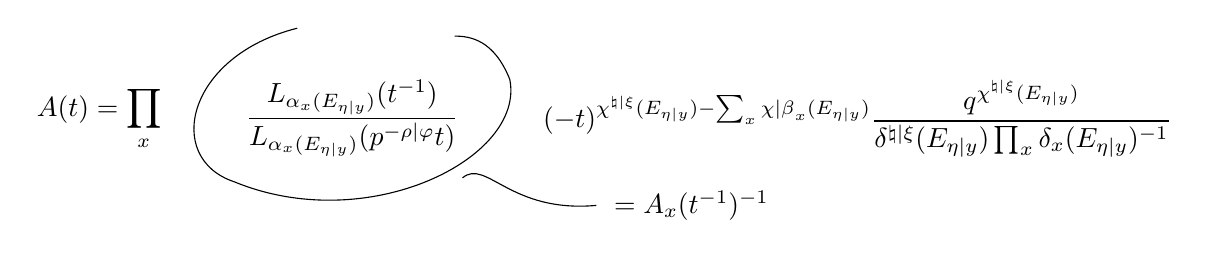
\begin{tikzpicture}[x=1cm,y=1cm]
\node[anchor=east] at (0,0) {$\displaystyle A(t)=\prod_x$};
\node at (2.3,0) {$\displaystyle\frac{L_{\alpha_x(E_{\unsure{\eta|y}})}(t^{-1})}{L_{\alpha_x(E_{\unsure{\eta|y}})}(p^{-\unsure{\rho|\varphi}}t)}$};
\node[anchor=west] at (4.6,0) {$\displaystyle(-t)^{\chi^{\unsure{\natural|\xi}}(E_{\unsure{\eta|y}})-\sum_x\unsure{\chi|\beta}_x(E_{\unsure{\eta|y}})}\frac{q^{\chi^{\unsure{\natural|\xi}}(E_{\unsure{\eta|y}})}}{\delta^{\unsure{\natural|\xi}}(E_{\unsure{\eta|y}})\prod_x\delta_x(E_{\unsure{\eta|y}})^{-1}}$};
\draw (1.6,1.15) .. controls (0.2,0.8) and (-0.1,-0.5) .. (0.8,-0.8) .. controls (2.5,-1.5) and (4.5,-0.5) .. (4.3,0.5) .. controls (4.1,1) and (3.8,1.05) .. (3.6,1.05);
\draw (3.7,-0.75) .. controls (4,-0.5) and (4.3,-1.2) .. (5.4,-1.1);
\node[anchor=west] at (5.5,-1.1) {$=A_x(t^{-1})^{-1}$};
\end{tikzpicture}}

\[
L_{\alpha_x(E_{\unsure{\eta|y}})}\left(\frac1{p^{\unsure{\rho|\varphi}}t}\right)=A_x(t)L_{\alpha_x(E_{\unsure{\eta|y}})}(t)
\]
\deleted{$\unsure{L_{\alpha_x(E)}}\quad L_{\alpha_x(E_{\unsure{\eta|y}})}($}

N.B. Ayant \unsure{coupé} $\lambda_x(\deleted{\unsure{\mu E}}\inserted{E_{\unsure{\eta|y}}})(t)$ \deleted{\unsure{en}} en \unsure{morceaux} ; on en perd le \uline{caractère additif}, Il vaut sans doute mieux ne pas \unsure{forcer} l'expression

\uline{Pb} a) Dans les cas géométriques classiques, construire les $\alpha_x(E_{\unsure{\eta|y}})$ pour déterminer les $\mu_x$, donc les $\lambda_x(E_{\unsure{\eta|y}})(t)$.
\diagram{\begin{tikzcd}[column sep=small,row sep=large]
\text{Déterminer en particulier} & \unsure{\chi|\beta}_x(E_{\unsure{\eta|y}}),\arrow[d,bend right] & \delta_x(E_{\unsure{\eta|y}}),\arrow[d,bend left]\\
\text{\parbox{7cm}{les \unsure{valeurs absolues} des \unsure{val.} propres de \unsure{Frobenius}.}} & \begin{gathered}\text{\unsure{invariant}}\\\text{\uuline{géom.}}\end{gathered} & \begin{gathered}\text{\unsure{invariant}}\\\text{\uuline{arithm.}}\end{gathered}\\
\text{\parbox{7cm}{b) Donner une formule genre \unsure{Chafarevitch} - Ogg pour}} & \chi^{\unsure{\natural|\xi}}(E_{\unsure{\eta|y}})\arrow[u,bend right] & \\
\text{c) Donner une formule pour} & & \delta^{\unsure{\natural|\xi}}(E_{\unsure{\eta|y}})\arrow[uu,bend right]
\end{tikzcd}}

\margin{54}
